\documentclass[a4paper,11pt,spanish, twoside, leqno]{tfg-uam}

\usepackage[utf8]{inputenc}
\usepackage{amsfonts, amssymb, amsmath, amsthm}
\usepackage{graphicx}
\usepackage{color}
\usepackage{xcolor}
\usepackage{tikz}
\usepackage{listofitems} % for \readlist to create arrays
\usepackage{hyperref}

\tikzstyle{mynode}=[thick,draw=blue,fill=blue!20,circle,minimum size=22]

\newtheorem{teor}{Teorema}[chapter]
\newtheorem{lema}[teor]{Lema}
\newtheorem*{teorsin}{Teorema}


\theoremstyle{definition}
\newtheorem{defin}[teor]{Definici\'on}

\title{Redes Neuronales: aproximación de EDPs}
\author{Luis Hebrero Garicano}
\tutor{Julia Novo}
\curso{2024-2025}


%%%%%METADATOS: rellenar la info solicitada entre llaves
\usepackage{hyperref}
\hypersetup{
	pdfinfo={
            Title={Redes Neuronales: aproximacion de EDPs}, %Titulo del trabajo; ejemplo: Matematicas y desarrollo
            Author={Luis Hebrero Garicano}, %Autor del trabajo; ejemplo: Juan Sanchez
            Director1={julia.novo}, %Tutor1: en formato nombre.apellido, tal como aparece en la primera parte, antes de la arroba,  de su direcci�n de correo electr�nico de la UAM; ejemplo: fernando.soria
            Director2={ }, %Tutor2: en formato nombre.apellido, tal como aparece en la primera parte, antes de la arroba,  de su direcci�n de correo electr�nico de la UAM
            Ndirectores={1}, %Numero total de directores: 1 � 2
            Tipo={TFG}, %no tocar
            Curso={2024-25}, %no tocar
            Palabrasclave={ },% Palabras clave del trabajo, separadas por comas y sin acentos ni espacios; ejemplo: morfismos, formas modulares, ecuaciones elipticas
				}
}
%%%%%%%%%%%%%%%%%%%%%%%%%%%%%%%

\begin{document}



\begin{abstract}[spanish]
Las redes neuronales son un modelo matemático inspirado en el funcionamiento cerebral que, en esencia, se utiliza para encontrar funciones: funciones que clasifican datos, que predicen valores o incluso que anticipan la siguiente palabra en una frase. En este trabajo, se estudiará cómo se puede aplicar esta capacidad de aproximación de funciones para resolver ecuaciones en derivadas parciales. Exploraremos distintas estrategias para construir estas redes y analizaremos su aplicación en problemas concretos, centrándonos en las ventajas que aportan con respecto a los métodos numéricos tradicionales, así como en los casos en los que una aproximación mediante redes neuronales no resulta efectiva.
\end{abstract}
\begin{abstract}[english]
Neural networks are a mathematical model inspired by the brain's functioning, primarily used to find functions: functions that classify data, predict values, or even anticipate the next word in a sentence. This work will explore how this function approximation capability can be applied to solve partial differential equations. We will investigate different strategies for constructing these networks and analyze their application to specific problems, focusing on the advantages they offer over traditional numerical methods, as well as the cases where a neural network-based approach proves ineffective.
\end{abstract}
\mainmatter


\chapter{Introducción y preliminares}\label{chap1}
\setcounter{page}{1}
Para poder entender el las aproximaciones a las EDPs mediante redes neuronales, es necesario tener un conocimiento previo de las redes neuronales y de las ecuaciones en derivadas parciales. En este capítulo, se introducirán los conceptos básicos de ambos temas, así como las herramientas matemáticas necesarias para comprender el resto del trabajo.

\section{Introducción a las redes neuronales}
Una red neuronal, de forma abstracta, es simplemente una función que toma una entrada y produce una salida. Es decir, una red neuronal, es una función $F$ que toma un vector de entrada $x$ y produce un vector de salida $y$, siendo $F: \mathbb{R}^n \rightarrow \mathbb{R}^m$. La red neuronal se compone de una serie de capas, cada una de las cuales está formada por un conjunto de neuronas. Cada neurona de una capa recibe una serie de entradas, las procesa y produce una salida. La salida de cada neurona se calcula mediante una función de activación, que puede ser de distintos tipos, como la función sigmoide, la función tangente hiperbólica o la función ReLU. Para entender este concepto nos vamos a centrar en el caso concreto de la red neuronal de la Figura \ref{fig:RedNeuronal}.


\begin{figure}[!ht]
    \centering
    \begin{tikzpicture}[x=2.2cm,y=1.4cm]
        \readlist\Nnod{2,2,3,3} % number of nodes per layer
        \readlist\colors{mylightred, mylightblue, mylightblue, mylightgreen} % color of each layer
        % \Nnodlen = length of \Nnod (i.e. total number of layers)
        % \Nnod[1] = element (number of nodes) at index 1
        \foreachitem \N \in \Nnod{ % loop over layers
          % \N     = current element in this iteration (i.e. number of nodes for this layer)
          % \Ncnt  = index of current layer in this iteration
          \foreach \i [evaluate={\x=\Ncnt; \y=\N/2-\i+0.5; \prev=int(\Ncnt-1);}] in {1,...,\N}{ % loop over nodes
            \node[mynode] (N\Ncnt-\i) at (\x,\y) {};
            \ifnum\Ncnt>1 % connect to previous layer
              \foreach \j in {1,...,\Nnod[\prev]}{ % loop over nodes in previous layer
                \draw[thick] (N\prev-\j) -- (N\Ncnt-\i); % connect arrows directly
              }
            \fi % else: nothing to connect first layer
          }
        }
    \end{tikzpicture}
    \caption{Esquema de una red neuronal con 4 capas.}
    \label{fig:RedNeuronal}
\end{figure}

Como se ve en la Figura \ref{fig:RedNeuronal}, la entrada en nuestra función está representada por los dos círculos de la izquierda, que representan los valores de entrada $x_1$ y $x_2$, siendo así la entrada $x\in\mathbb{R}^2$. Estos valores se multiplican por unos pesos ($W^{[2]}$)y se suman a un sesgo $b$. La salida de esta neurona se calcula mediante una función de activación. Así, los valores que ``llegan'' a la segunda capa de nuestra red neuronal serán de la forma
\begin{equation*}
    \sigma(W^{[2]}x+b^{[2]})\in\mathbb{R}^2,
\end{equation*}

Siendo $W^{[2]}\in\mathbb{R}^{2\times2}$ y el vector $b^{[2]}\in\mathbb{R}^2$. A partir de aquí, se repite el proceso para cada capa de la red neuronal, hasta llegar a la capa de salida, que nos dará el valor de salida de nuestra red neuronal. De forma visual, se pueden interpretar las flechas de la Figura \ref{fig:RedNeuronal} como los pesos por los que se va multiplicando.

En la tercera capa de la red neuronal, vemos que los valores que llegan de la capa 2, estos $\sigma(W^{[2]}x+b^{[2]})$, pertenecen a $\mathbb{R}^2$. De este modo, como tenemos 3 neuronas en la tercera capa, para obtener un valor perteneciente a $\mathbb{R}^3$, necesitamos una matriz $W^{[3]}\in\mathbb{R}^{3\times2}$ y un vector $b^{[3]}\in\mathbb{R}^3$. Así, el valor de nuestra red neuronal en la tercera capa será
\begin{equation*}
    \sigma(W^{[3]}\sigma(W^{[2]}x+b^{[2]})+b^{[3]})\in\mathbb{R}^3.
\end{equation*}

Finalmente, la capa de salida recibirá de la tercera capa un vector perteneciente a $\mathbb{R}^3$, por lo que necesitaremos una matriz $W^{[4]}\in\mathbb{R}^{3\times3}$ y un vector $b^{[4]}\in\mathbb{R}^3$. Así, el valor de salida de nuestra red neuronal, esa $F$ de la que habíamos hablado al principio, será
\begin{equation}
    F(x)=\sigma(W^{[4]}\sigma(W^{[3]}\sigma(W^{[2]}x+b^{[2]})+b^{[3]})+b^{[4]})\in\mathbb{R}^3.
\end{equation}\label{eq:RedNeuronal}

En general, una red neuronal se puede representar como una composición de funciones, donde cada función es una capa de la red neuronal. 

Nuestra intención con este tipo de funciones es ir variando los valores de las matrices $W$, también conocidos como pesos, y los vectores $b$ también conocidos como sesgos, para que la salida de nuestra red neuronal se acerque lo máximo posible a la salida deseada. 

Para entender esto, vamos a utilizar la red neuronal de la Figura \ref{fig:RedNeuronal} para resolver un problema concreto muy sencillo de clasificación. Supongamos que tenemos una serie de puntos en el plano, de tres tipos distintos, como los de la Figura \ref{fig:Clasificacion}, y queremos clasificarlos en tres grupos, los puntos de tipo azul, rojo y amarillo.


\begin{figure}[!ht]
    \centering
    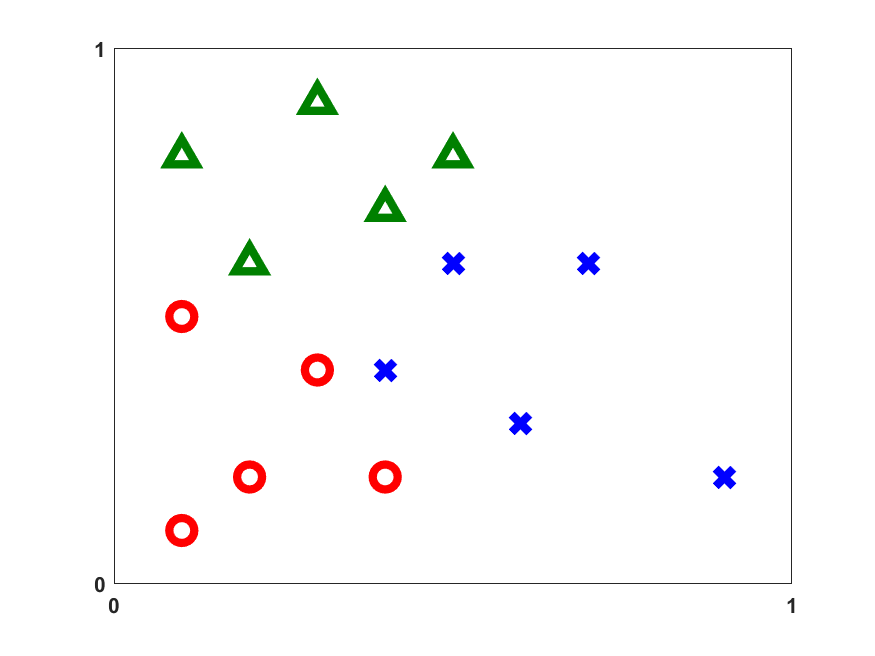
\includegraphics[width=0.5\textwidth]{Figuras/pic_xy.png}
    \caption{Puntos en el plano que marcan las dos categorías}
    \label{fig:Clasificacion}
\end{figure}

De este modo, nuestra red neuronal recivirá como entrada un punto del plano, y nos dirá a qué categoría pertenece, devolviendo $(1,0,0)^T$ si es de la categoría azul, $(0,1,0)^T$ si es de la categoría roja y $(0,0,1)^T$ si es de la categoría amarilla.

Lo siguiente que queremos hacer será entrenar la red neuronal, es decir, ajustar los pesos y sesgos de la red neuronal para que la salida se acerque lo máximo posible a la salida deseada. Es decir, que cuando se introduzca un punto de un tipo concreto, la salida lo asigne a la categoría adecuada. 

Designamos a $y(x)$ como la salida deseada de nuestra red neuronal, y a $F(x)$ como la salida real. Así, el error vendrá dado en función de los pesos y sesgos de la siguiente forma
\begin{equation*}
    E(W^{[2]},W^{[3]},W^{[4]},b^{[2]},b^{[3]},b^{[4]})=\frac{1}{2}\sum_{x\in X}\|y(x)-F(x)\|^2,
\end{equation*}

Donde $X$ es el conjunto de puntos que tenemos para entrenar la red neuronal, en nuestro caso, serán 15. Así, lo que queremos hacer es minimizar esta función de error, es decir, encontrar los pesos que minimicen la función $E$. Para ello, se utilizan algoritmos de optimización, como el descenso del gradiente. Este proceso es conocido como el entrenamiento de la red neuronal. Si se logra con éxito, la red neuronal será capaz de clasificar correctamente los puntos en el plano. En este caso concreto, al entrenar la red neuronal, se obtiene la clasificación de la Figura \ref{fig:ClasificacionFinal}, en la que simplemente hemos aplicado nuestra función para cada punto del plano y lo hemos sombreado de acuerdo a la clasificación que se le ha dado.

\begin{figure}[!ht]
    \centering
    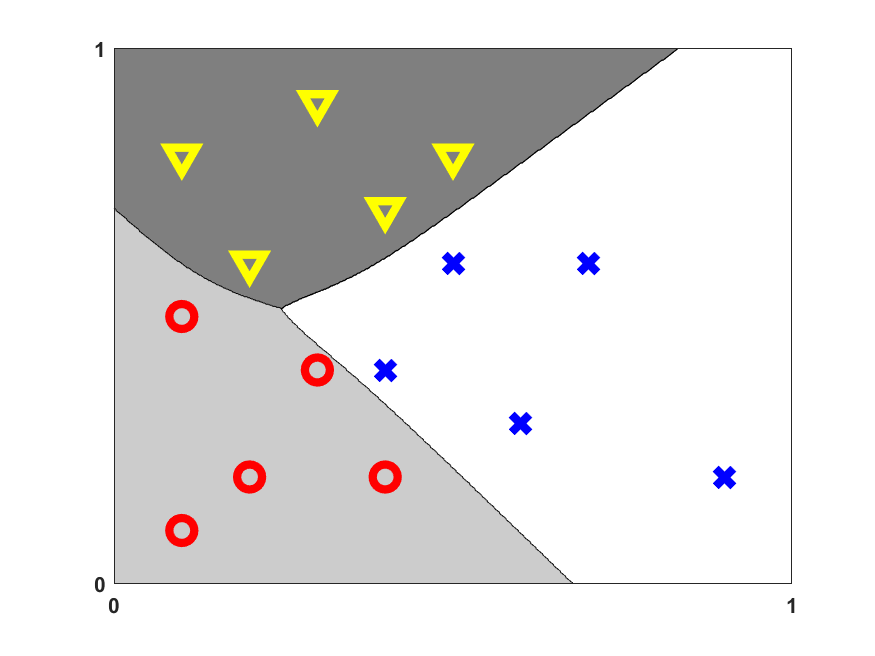
\includegraphics[width=0.5\textwidth]{Figuras/classifier_back.png}
    \caption{Puntos en el plano que marcan las dos categorías}
    \label{fig:ClasificacionFinal}
\end{figure}

Más adelante entenderemos con más detalle como es este proceso de entrenamiento.

\subsection{Comentarios sobre la función sigmoide}
Como hemos visto con el ejemplo anterior, las redes neuronales se pueden utilizar para generar funciones. A su vez, estas funciones se utilizan para resolver problemas de forma aproximada. En el ejemplo de la Figura \ref{fig:RedNeuronal}, la función red neuronal clasifica cualquier parte del plano en una de las tres categorías sombreadas a partir del entrenamiento. Dicho entrenamiento fija los valores de los pesos y sesgos, y por tanto define la funcion rede neuronal (en el ejemplo define la funcion \ref{eq:RedNeuronal}).

Como las redes neuronales se utilizan para aproximar problemas de tipos muy distintos, una de las características deseables es que sean  capaces de aproximar el conjunto de funciones "mayor posible".

Para poder lograr este objetivo, se necesitan las funciones de activación. Como ejercicio, supongamos que en nuestra ecuación \ref{eq:RedNeuronal} en lugar de utilizar la función sigmoide, no utilizamos ninguna función de activación, es decir, que nuestra red neuronal es simplemente una composición de funciones lineales. En este caso, nuestra red tendría la siguiente forma

\begin{equation*}
    F(x)=W^{[4]}(W^{[3]}(W^{[2]}x+b^{[2]})+b^{[3]})+b^{[4]}\in\mathbb{R}^3.
\end{equation*}

Claramente, una función lineal definida de forma global puede estar muy lejos de aproximar bien funciones generales. De este modo, parece por tanto razonables utilizar funciones de activación no lineales. La función sigmoide es una de las más utilizadas, pero existen otras como la función tangente hiperbólica o la función ReLU. En este trabajo, nos centraremos en la función sigmoide, que se define como
\begin{equation*}
    \sigma(x)=\frac{1}{1+e^{-x}}.
\end{equation*}

Esta función tiene la ventaja de que su derivada es fácil de calcular, y es precisamente esta derivada la que se utiliza en el algoritmo de entrenamiento de la red neuronal.

Un resultado relevante para justificar el uso de funciones de activación no lineales es el siguiente es el propuesto por Pinkus\cite{Pinkus}. Este resultado es para neuronales de una sola capa, no obstante, si se cumple en una sola capa, es trivial la extensión a $n$ capas.

\begin{teor}[Pinkus]
    Sea $\sigma\in C(\mathbb{R})$ y sea conjunto $\mathcal{M}(\sigma) = \text{span}\{\sigma(w\cdot x + b): b \in \mathbb{R}, w \in \mathbb{R}^n\}$, se cumple que
    
    Para cualquier $f \in C(\mathbb{R}^n)$, cualquier conjunto compacto $K\in \mathbb{R}^n$ y cualquier $\epsilon > 0$, existe una funcion $g\in \mathcal{M}(\sigma)$ tal que $\max_{x\in K}|f(x)-g(x)|<\epsilon$. Si y solo si $\sigma$ no es una función polinómica.
\end{teor}
De forma más intuitva, cualquier función $f \in C(\mathbb{R}^n)$, se puede aproximar tan bien como se quiera con una red neuronal de una sola capa si y solo si la función de activación no es polinómica.

Este resultado nos aporta una intuición de por qué las funciones de activación no lineales son necesarias para aproximar funciones de forma general pues, de nos ser funciones no lineales, habría muchas funciones que no podríamos aproximar. 

\section{Introducción a las ecuaciones en derivadas parciales}

Las ecuaciones en derivadas parciales (EDPs) son ecuaciones que relacionan una función desconocida con sus derivadas parciales. Son fundamentales en la física y en la ingeniería, ya que permiten modelar fenómenos físicos y predecir su evolución en el tiempo. 

Existen varios tipos de EDPs, no obstante, nosotros nos centraremos en las ecuación ellipticas. Estas se utilizan para resolver problemas de equilibrio, que implican encontrar la solución de una ecuación diferencial en un dominio cerrado con condiciones de frontera específicas. Estos problemas incluyen la distribución estacionaria de temperatura, el flujo de fluidos incompresibles no viscosos, la distribución de tensiones en sólidos en equilibrio, y el cálculo de campos eléctricos en regiones con densidad de carga. En general, se aplican cuando se busca determinar un potencial en situaciones estacionarias. 

Lo he sacado de aquí \href{https://www.ugr.es/~prodelas/ftp/ETSICCP/Resoluci%F3nNum%E9ricaEDPs.pdf}{Este enlace, \colorbox{yellow}{este tipo de cosas se citan?}}


%se puede hablar de los espacios de funciones en los que trabajamos, que es el supp de una función. Poner un ejemplo de ecuación diferencial y por que no se puede encontrar su solución en forma fuerte

\begin{equation*}
    \nabla u = 0,
\end{equation*}




\section{Forma fuerte y débil de una EDP}
%Introducir la idea y usar el ejemplo del apartado anterior par ademostrar que no todas las ecuciones en forma fuerte tienen solución
Una ecuación en derivadas parciales se puede escribir en forma fuerte o en forma débil. La forma fuerte de una ecuación en derivadas parciales es una ecuación diferencial que relaciona la función desconocida con sus derivadas parciales. Por ejemplo, la ecuación de Poisson, que modela la distribución de temperatura en un sólido, se puede escribir en forma fuerte como


%quiza tenga sentido hablar de que ni siquiera en forma debil se puede encontrar la solución, y que por eso se recurre a métodos alternativos (metodos numéricos)

%también puede tener sentido hablar de las ecuaciones en las que la solucion es el mínimo de una funcion, y que por eso se puede resolver con redes neuronales

\section{Métodos numéricos tradicionales: el método de los elementos finitos}
% hablar de como funciona en detalle, 
El método de los elementos finitos es uno de los métodos numéricos más utilizados para resolver ecuaciones en derivadas parciales. Consiste en dividir el dominio de la ecuación en un conjunto de elementos finitos, y aproximar la solución de la ecuación en cada elemento mediante una función polinómica. La solución de la ecuación se obtiene entonces como una combinación lineal de las soluciones en cada elemento. El método de los elementos finitos es muy eficaz para resolver ecuaciones en derivadas parciales elípticas, pero presenta algunas limitaciones, como la necesidad de discretizar el dominio de la ecuación y la dificultad de tratar con geometrías complejas. En este trabajo, exploraremos cómo las redes neuronales pueden superar estas limitaciones y proporcionar una alternativa eficaz y flexible para resolver ecuaciones en derivadas parciales.
\colorbox{yellow}{Todo lo que sea necesario para poder entender el resto del trabajo.}

\chapter{Aproximación de EDPs mediante redes neuronales}\label{chap2}

\section{PINS }
\section{El ``Deep Ritz Method''}

\chapter{Resultados}\label{chap3}





\headrule
\newpage
\section{Notas del formato}
\begin{teorsin}
[Cauchy--Schwarz]Nullam quis ante. 
\end{teorsin}

\begin{teor}\label{teor1}
Nullam quis ante. Etiam sit amet orci eget eros faucibus tincidunt. Duis leo. Sed fringilla mauris sit amet nibh. Donec sodales sagittis magna. Sed consequat, leo eget bibendum sodales, augue velit cursus nunc.
\end{teor}

\begin{defin}
Nullam quis ante. Etiam sit amet orci eget eros faucibus tincidunt. Duis leo. Sed fringilla mauris sit amet nibh. Donec sodales sagittis magna. Sed consequat, leo eget bibendum sodales, augue velit cursus nunc.
\end{defin}
\begin{lema}\label{lema1}
Nullam quis ante. Etiam sit amet orci eget eros faucibus tincidunt. Duis leo. Sed fringilla mauris sit amet nibh. Donec sodales sagittis magna. Sed consequat, leo eget bibendum sodales, augue velit cursus nunc.
\end{lema}
\begin{proof}
Nullam quis ante. 
\end{proof}


\begin{lema}\label{lema2}
Nullam quis ante. Etiam sit amet orci eget eros faucibus tincidunt. Duis leo. Sed fringilla mauris sit amet nibh. Donec sodales sagittis magna. Sed consequat, leo eget bibendum sodales, augue velit cursus nunc.
\end{lema}

Lorem ipsum dolor sit amet, consectetuer adipiscing elit. Aenean commodo ligula eget dolor. Aenean massa. Cum sociis natoque penatibus et magnis dis parturient montes, nascetur ridiculus mus. Donec quam felis, ultricies nec, pellentesque eu, pretium quis, sem. Nulla consequat massa quis enim. Donec pede justo, fringilla vel, aliquet nec, vulputate eget, arcu. In enim justo, rhoncus ut, imperdiet a, venenatis vitae, justo. Nullam dictum felis eu pede mollis pretium. Integer tincidunt. Cras dapibus. Vivamus elementum semper nisi. Aenean vulputate eleifend tellus. Aenean leo ligula, porttitor eu, consequat vitae, eleifend ac, enim. Aliquam lorem ante, dapibus in, viverra quis, feugiat a, tellus. Phasellus viverra nulla ut metus varius laoreet. Quisque rutrum. Aenean imperdiet. Etiam ultricies nisi vel augue. Curabitur ullamcorper ultricies nisi. Nam eget dui. Etiam rhoncus. Maecenas tempus, tellus eget condimentum rhoncus, sem quam semper libero, sit amet adipiscing sem neque sed ipsum. Nam quam nunc, blandit vel, luctus pulvinar, hendrerit id, lorem. Maecenas nec odio et ante tincidunt tempus. Donec vitae sapien ut libero venenatis faucibus. Nullam quis ante. Etiam sit amet orci eget eros faucibus tincidunt. Duis leo. Sed fringilla mauris sit amet nibh. Donec sodales sagittis magna. Sed consequat, leo eget bibendum sodales, augue velit cursus nunc.


\begin{proof}[\sc Demostraci\'on del lema {\rm \ref{lema2}}]
Nullam quis ante:
\begin{equation}
2+2=4.\qedhere
\end{equation}
\end{proof}

Lorem ipsum dolor sit amet, Teorema \ref{teor1}, consectetuer adipiscing elit. Aenean commodo ligula eget dolor. Aenean massa. Cum sociis natoque penatibus et magnis dis parturient montes, nascetur ridiculus mus. Donec quam felis, ultricies nec, pellentesque eu, pretium quis, sem. Nulla consequat massa quis enim. Donec pede justo, fringilla vel, aliquet nec, vulputate eget, arcu. In enim justo, rhoncus ut, imperdiet a, venenatis vitae, justo. Nullam dictum felis eu pede mollis pretium. Integer tincidunt. Cras dapibus. Vivamus elementum semper nisi. Aenean vulputate eleifend tellus. Aenean leo ligula, porttitor eu, consequat vitae, eleifend ac, enim. Aliquam lorem ante, dapibus in, viverra quis, feugiat a, tellus. Phasellus viverra nulla ut metus varius laoreet. Quisque rutrum. Aenean imperdiet. Etiam ultricies nisi vel augue. Curabitur ullamcorper ultricies nisi. Nam eget dui. Etiam rhoncus. Maecenas tempus, tellus eget condimentum rhoncus, sem quam semper libero, sit amet adipiscing sem neque sed ipsum. Nam quam nunc, blandit vel, luctus pulvinar, hendrerit id, lorem. Maecenas nec odio et ante tincidunt tempus. Donec vitae sapien ut libero venenatis faucibus. Nullam quis ante. Etiam sit amet orci eget eros faucibus tincidunt. Duis leo. Sed fringilla mauris sit amet nibh. Donec sodales sagittis magna. Sed consequat, leo eget bibendum sodales, augue velit cursus nunc,
\begin{align}\label{eq4}
&e^{i\pi }+1=0,
\\
&2e^{i\pi }+2=0.\label{eq5}
\end{align}

Lorem ipsum dolor sit amet, consectetuer adipiscing elit. Aenean commodo ligula eget dolor.
\begin{align}\nonumber
0&=e^{i\pi }+1=e^{i\pi }+1=e^{i\pi }+1=e^{i\pi }+\sum_{n=1}^\infty \frac{1}{2^n}
\\
&=-1+\sum_{n=1}^\infty \frac{1}{2^n}=-1+1=0.\label{eq6}
\end{align}
et
\begin{equation}\label{eq7}
\begin{aligned}
e^{i\pi }+1=0,
\\
e^{i\pi }+1=0.
\end{aligned}
\end{equation}


Lorem ipsum dolor sit amet, consectetuer adipiscing elit. Aenean commodo ligula eget dolor.
\begin{align*}
e^{i\pi }+1&=0,
\\
e^{i\pi }+1&=0.
\end{align*}
Aenean massa: 
\begin{equation}
\left\{
\begin{array}{l}
e^{i\pi }+1=0,
\\
e^{i\pi }+1=0.
\end{array}
\right.
\end{equation}


Cum sociis natoque penatibus et magnis dis parturient montes, nascetur ridiculus mus. Donec quam felis, ultricies nec, pellentesque eu, pretium quis, sem. Nulla consequat massa quis enim. Donec pede justo, fringilla vel, aliquet nec, vulputate eget, arcu. In enim justo, rhoncus ut, imperdiet a, venenatis vitae, justo. Nullam dictum felis eu pede mollis pretium. Integer tincidunt. Cras dapibus. Vivamus elementum semper nisi. Aenean vulputate eleifend tellus. Aenean leo ligula, porttitor eu, consequat vitae, eleifend ac, enim. Aliquam lorem ante, dapibus in, viverra quis, feugiat a, tellus. Phasellus viverra nulla ut metus varius laoreet. Quisque rutrum. Aenean imperdiet. Etiam ultricies nisi vel augue. Curabitur ullamcorper ultricies nisi. Nam eget dui. Etiam rhoncus. Maecenas tempus, tellus eget condimentum rhoncus, sem quam semper libero, sit amet adipiscing sem neque sed ipsum. Nam quam nunc, blandit vel, luctus pulvinar, hendrerit id, lorem. Maecenas nec odio et ante tincidunt tempus. Donec vitae sapien ut libero venenatis faucibus. Nullam quis ante. Etiam sit amet orci eget eros faucibus tincidunt. Duis leo. Sed fringilla mauris sit amet nibh. Donec sodales sagittis magna. Sed consequat, leo eget bibendum sodales, augue velit cursus nunc,

Lorem ipsum dolor sit amet, consectetuer adipiscing elit. Aenean commodo ligula eget dolor. Aenean massa. Cum sociis natoque penatibus et magnis dis parturient montes, nascetur ridiculus mus. Donec quam felis, ultricies nec, pellentesque eu, pretium quis, sem. Nulla consequat massa quis enim. Donec pede justo, fringilla vel, aliquet nec, vulputate eget, arcu. In enim justo, rhoncus ut, imperdiet a, venenatis vitae, justo. Nullam dictum felis eu pede mollis pretium. Integer tincidunt. Cras dapibus. Vivamus elementum semper nisi. Aenean vulputate eleifend tellus. Aenean leo ligula, porttitor eu, consequat vitae, eleifend ac, enim. Aliquam lorem ante, dapibus in, viverra quis, feugiat a, tellus. Phasellus viverra nulla ut metus varius laoreet. Quisque rutrum. Aenean imperdiet. Etiam ultricies nisi vel augue. Curabitur ullamcorper ultricies nisi. Nam eget dui. Etiam rhoncus. Maecenas tempus, tellus eget condimentum rhoncus, sem quam semper libero, sit amet adipiscing sem neque sed ipsum. Nam quam nunc, blandit vel, luctus pulvinar, hendrerit id, lorem. Maecenas nec odio et ante tincidunt tempus. Donec vitae sapien ut libero venenatis faucibus. Nullam quis ante. Etiam sit amet orci eget eros faucibus tincidunt. Duis leo. Sed fringilla mauris sit amet nibh. Donec sodales sagittis magna. Sed consequat, leo eget bibendum sodales, augue velit cursus nunc,


\chapter{El segundo cap\'{\i}tulo}\label{chap4}

Lorem ipsum dolor sit amet, consectetuer adipiscing elit. Aenean commodo ligula eget dolor. Aenean massa. Cum sociis natoque penatibus et magnis dis parturient montes, nascetur ridiculus mus. Donec quam felis, ultricies nec, pellentesque eu, pretium quis, sem. Nulla consequat massa quis enim. Donec pede justo, fringilla vel, aliquet nec, vulputate eget, arcu. In enim justo, rhoncus ut, imperdiet a, venenatis vitae, justo. Nullam dictum felis eu pede mollis pretium. Integer tincidunt. Cras dapibus. Vivamus elementum semper nisi. Aenean vulputate eleifend tellus. Aenean leo ligula, porttitor eu, consequat vitae, eleifend ac, enim. Aliquam lorem ante, dapibus in, viverra quis, feugiat a, tellus.
\begin{equation}\label{eq8}
e^{i\pi }+1=0.
\end{equation}
Phasellus viverra nulla ut metus varius laoreet. Quisque rutrum. Aenean imperdiet. Etiam ultricies nisi vel augue. Curabitur ullamcorper ultricies nisi. Nam eget dui. Etiam rhoncus. Maecenas tempus, tellus eget condimentum rhoncus, sem quam semper libero, sit amet adipiscing sem neque sed ipsum. Nam quam nunc, blandit vel, luctus pulvinar, hendrerit id, lorem. Maecenas nec odio et ante tincidunt tempus. Donec vitae sapien ut libero venenatis faucibus. Nullam quis ante. Etiam sit amet orci eget eros faucibus tincidunt. Duis leo. Sed fringilla mauris sit amet nibh. Donec sodales sagittis magna. Sed consequat, leo eget bibendum sodales, augue velit cursus nunc,
$$
e^{i\pi }+1=0.
$$

Lorem ipsum dolor sit amet, consectetuer adipiscing elit. Aenean commodo ligula eget dolor. Aenean massa. Cum sociis natoque penatibus et magnis dis parturient montes, nascetur ridiculus mus. Donec quam felis, ultricies nec, pellentesque eu, pretium quis, sem. Nulla consequat massa quis enim. Donec pede justo, fringilla vel, aliquet nec, vulputate eget, arcu. In enim justo, rhoncus ut, imperdiet a, venenatis vitae, justo. Nullam dictum felis eu pede mollis pretium.
\begin{equation}
e^{i\pi }+1=0.
\end{equation}


Integer tincidunt. Cras dapibus. Vivamus elementum semper nisi. Aenean vulputate eleifend tellus. Aenean leo ligula, porttitor eu, consequat vitae, eleifend ac, enim. Aliquam lorem ante, dapibus in, viverra quis, feugiat a, tellus. Phasellus viverra nulla ut metus varius laoreet. Quisque rutrum. Aenean imperdiet. Etiam ultricies nisi vel augue. Curabitur ullamcorper ultricies nisi.
\begin{equation}
e^{i\pi }+1=0.
\end{equation}
Nam eget dui. Etiam rhoncus. Maecenas tempus, tellus eget condimentum rhoncus, sem quam semper libero, sit amet adipiscing sem neque sed ipsum. Nam quam nunc, blandit vel, luctus pulvinar, hendrerit id, lorem. Maecenas nec odio et ante tincidunt tempus. Donec vitae sapien ut libero venenatis faucibus. Nullam quis ante. Etiam sit amet orci eget eros faucibus tincidunt. Duis leo. Sed fringilla mauris sit amet nibh. Donec sodales sagittis magna. Sed consequat, leo eget bibendum sodales, augue velit cursus nunc,
$$
e^{i\pi }+1=0.
$$

Lorem ipsum dolor sit amet, consectetuer adipiscing elit. Aenean commodo ligula eget dolor. Aenean massa. Cum sociis natoque penatibus et magnis dis parturient montes, nascetur ridiculus mus. Donec quam felis, ultricies nec, pellentesque eu, pretium quis, sem. Nulla consequat massa quis enim. Donec pede justo, fringilla vel, aliquet nec, vulputate eget, arcu. In enim justo, rhoncus ut, imperdiet a, venenatis vitae, justo. Nullam dictum felis eu pede mollis pretium. Integer tincidunt. Cras dapibus. Vivamus elementum semper nisi. Aenean vulputate eleifend tellus. Aenean leo ligula, porttitor eu, consequat vitae, eleifend ac, enim. Aliquam lorem ante, dapibus in, viverra quis, feugiat a, tellus. Phasellus viverra nulla ut metus varius laoreet. Quisque rutrum. Aenean imperdiet. Etiam ultricies nisi vel augue. Curabitur ullamcorper ultricies nisi. Nam eget dui. Etiam rhoncus. Maecenas tempus, tellus eget condimentum rhoncus, sem quam semper libero, sit amet adipiscing sem neque sed ipsum. Nam quam nunc, blandit vel, luctus pulvinar, hendrerit id, lorem. Maecenas nec odio et ante tincidunt tempus. Donec vitae sapien ut libero venenatis faucibus. Nullam quis ante. Etiam sit amet orci eget eros faucibus tincidunt. Duis leo. Sed fringilla mauris sit amet nibh. Donec sodales sagittis magna. Sed consequat, leo eget bibendum sodales, augue velit cursus nunc,

\section{Uno m\'as}

Lorem ipsum dolor sit amet, consectetuer adipiscing elit. Aenean commodo ligula eget dolor. Aenean massa. Cum sociis natoque penatibus et magnis dis parturient montes, nascetur ridiculus mus. Donec quam felis, ultricies nec, pellentesque eu, pretium quis, sem. Nulla consequat massa quis enim. Donec pede justo, fringilla vel, aliquet nec, vulputate eget, arcu. In enim justo, rhoncus ut, imperdiet a, venenatis vitae, justo. Nullam dictum felis eu pede mollis pretium. Integer tincidunt. Cras dapibus. Vivamus elementum semper nisi. Aenean vulputate eleifend tellus. Aenean leo ligula, porttitor eu, consequat vitae, eleifend ac, enim. Aliquam lorem ante, dapibus in, viverra quis, feugiat a, tellus. Phasellus viverra nulla ut metus varius laoreet. Quisque rutrum. Aenean imperdiet. Etiam ultricies nisi vel augue. Curabitur ullamcorper ultricies nisi. Nam eget dui. Etiam rhoncus. Maecenas tempus, tellus eget condimentum rhoncus, sem quam semper libero, sit amet adipiscing sem neque sed ipsum. Nam quam nunc, blandit vel, luctus pulvinar, hendrerit id, lorem. Maecenas nec odio et ante tincidunt tempus. Donec vitae sapien ut libero venenatis faucibus. Nullam quis ante. Etiam sit amet orci eget eros faucibus tincidunt. Duis leo. Sed fringilla mauris sit amet nibh. Donec sodales sagittis magna. Sed consequat, leo eget bibendum sodales, augue velit cursus nunc,
$$
e^{i\pi }+1=0.
$$

\section{Y otro}

Lorem ipsum dolor sit amet, consectetuer adipiscing elit. Aenean commodo ligula eget dolor. Aenean massa. Cum sociis natoque penatibus et magnis dis parturient montes, nascetur ridiculus mus. Donec quam felis, ultricies nec, pellentesque eu, pretium quis, sem. Nulla consequat massa quis enim. Donec pede justo, fringilla vel, aliquet nec, vulputate eget, arcu. In enim justo, rhoncus ut, imperdiet a, venenatis vitae, justo. Nullam dictum felis eu pede mollis pretium. Integer tincidunt. Cras dapibus. Vivamus elementum semper nisi. Aenean vulputate eleifend tellus. Aenean leo ligula, porttitor eu, consequat vitae, eleifend ac, enim. Aliquam lorem ante, dapibus in, viverra quis, feugiat a, tellus. Phasellus viverra nulla ut metus varius laoreet. Quisque rutrum. Aenean imperdiet. Etiam ultricies nisi vel augue. Curabitur ullamcorper ultricies nisi. Nam eget dui. Etiam rhoncus. Maecenas tempus, tellus eget condimentum rhoncus, sem quam semper libero, sit amet adipiscing sem neque sed ipsum. Nam quam nunc, blandit vel, luctus pulvinar, hendrerit id, lorem. Maecenas nec odio et ante tincidunt tempus. Donec vitae sapien ut libero venenatis faucibus. Nullam quis ante. Etiam sit amet orci eget eros faucibus tincidunt. Duis leo. Sed fringilla mauris sit amet nibh. Donec sodales sagittis magna. Sed consequat, leo eget bibendum sodales, augue velit cursus nunc,


Lorem ipsum dolor sit amet, consectetuer adipiscing elit. Aenean commodo ligula eget dolor. Aenean massa. Cum sociis natoque penatibus et magnis dis parturient montes, nascetur ridiculus mus. Donec quam felis, ultricies nec, pellentesque eu, pretium quis, sem. Nulla consequat massa quis enim. Donec pede justo, fringilla vel, aliquet nec, vulputate eget, arcu. In enim justo, rhoncus ut, imperdiet a, venenatis vitae, justo. Nullam dictum felis eu pede mollis pretium. Integer tincidunt. Cras dapibus. Vivamus elementum semper nisi. Aenean vulputate eleifend tellus. Aenean leo ligula, porttitor eu, consequat vitae, eleifend ac, enim. Aliquam lorem ante, dapibus in, viverra quis, feugiat a, tellus. Phasellus viverra nulla ut metus varius laoreet. Quisque rutrum. Aenean imperdiet. Etiam ultricies nisi vel augue. Curabitur ullamcorper ultricies nisi. Nam eget dui. Etiam rhoncus. Maecenas tempus, tellus eget condimentum rhoncus, sem quam semper libero, sit amet adipiscing sem neque sed ipsum. Nam quam nunc, blandit vel, luctus pulvinar, hendrerit id, lorem. Maecenas nec odio et ante tincidunt tempus. Donec vitae sapien ut libero venenatis faucibus. Nullam quis ante. Etiam sit amet orci eget eros faucibus tincidunt. Duis leo. Sed fringilla mauris sit amet nibh. Donec sodales sagittis magna. Sed consequat, leo eget bibendum sodales, augue velit cursus nunc,


Lorem ipsum dolor sit amet, consectetuer adipiscing elit. Aenean commodo ligula eget dolor. Aenean massa. Cum sociis natoque penatibus et magnis dis parturient montes, nascetur ridiculus mus. Donec quam felis, ultricies nec, pellentesque eu, pretium quis, sem. Nulla consequat massa quis enim. Donec pede justo, fringilla vel, aliquet nec, vulputate eget, arcu. In enim justo, rhoncus ut, imperdiet a, venenatis vitae, justo. Nullam dictum felis eu pede mollis pretium. Integer tincidunt. Cras dapibus. Vivamus elementum semper nisi. Aenean vulputate eleifend tellus. Aenean leo ligula, porttitor eu, consequat vitae, eleifend ac, enim. Aliquam lorem ante, dapibus in, viverra quis, feugiat a, tellus. Phasellus viverra nulla ut metus varius laoreet. Quisque rutrum. Aenean imperdiet. Etiam ultricies nisi vel augue. Curabitur ullamcorper ultricies nisi. Nam eget dui. Etiam rhoncus. Maecenas tempus, tellus eget condimentum rhoncus, sem quam semper libero, sit amet adipiscing sem neque sed ipsum. Nam quam nunc, blandit vel, luctus pulvinar, hendrerit id, lorem. Maecenas nec odio et ante tincidunt tempus. Donec vitae sapien ut libero venenatis faucibus. Nullam quis ante. Etiam sit amet orci eget eros faucibus tincidunt. Duis leo. Sed fringilla mauris sit amet nibh. Donec sodales sagittis magna. Sed consequat, leo eget bibendum sodales, augue velit cursus nunc,


Lorem ipsum dolor sit amet, consectetuer adipiscing elit. Aenean commodo ligula eget dolor. Aenean massa. Cum sociis natoque penatibus et magnis dis parturient montes, nascetur ridiculus mus. Donec quam felis, ultricies nec, pellentesque eu, pretium quis, sem. Nulla consequat massa quis enim. Donec pede justo, fringilla vel, aliquet nec, vulputate eget, arcu. In enim justo, rhoncus ut, imperdiet a, venenatis vitae, justo. Nullam dictum felis eu pede mollis pretium. Integer tincidunt. Cras dapibus. Vivamus elementum semper nisi. Aenean vulputate eleifend tellus. Aenean leo ligula, porttitor eu, consequat vitae, eleifend ac, enim. Aliquam lorem ante, dapibus in, viverra quis, feugiat a, tellus. Phasellus viverra nulla ut metus varius laoreet. Quisque rutrum. Aenean imperdiet. Etiam ultricies nisi vel augue. Curabitur ullamcorper ultricies nisi. Nam eget dui. Etiam rhoncus. Maecenas tempus, tellus eget condimentum rhoncus, sem quam semper libero, sit amet adipiscing sem neque sed ipsum. Nam quam nunc, blandit vel, luctus pulvinar, hendrerit id, lorem. Maecenas nec odio et ante tincidunt tempus. Donec vitae sapien ut libero venenatis faucibus. Nullam quis ante. Etiam sit amet orci eget eros faucibus tincidunt. Duis leo. Sed fringilla mauris sit amet nibh. Donec sodales sagittis magna. Sed consequat, leo eget bibendum sodales, augue velit cursus nunc,


Lorem ipsum dolor sit amet, consectetuer adipiscing elit. Aenean commodo ligula eget dolor. Aenean massa. Cum sociis natoque penatibus et magnis dis parturient montes, nascetur ridiculus mus. Donec quam felis, ultricies nec, pellentesque eu, pretium quis, sem. Nulla consequat massa quis enim. Donec pede justo, fringilla vel, aliquet nec, vulputate eget, arcu. In enim justo, rhoncus ut, imperdiet a, venenatis vitae, justo. Nullam dictum felis eu pede mollis pretium. Integer tincidunt. Cras dapibus. Vivamus elementum semper nisi. Aenean vulputate eleifend tellus. Aenean leo ligula, porttitor eu, consequat vitae, eleifend ac, enim. Aliquam lorem ante, dapibus in, viverra quis, feugiat a, tellus. Phasellus viverra nulla ut metus varius laoreet. Quisque rutrum. Aenean imperdiet. Etiam ultricies nisi vel augue. Curabitur ullamcorper ultricies nisi. Nam eget dui. Etiam rhoncus. Maecenas tempus, tellus eget condimentum rhoncus, sem quam semper libero, sit amet adipiscing sem neque sed ipsum. Nam quam nunc, blandit vel, luctus pulvinar, hendrerit id, lorem. Maecenas nec odio et ante tincidunt tempus. Donec vitae sapien ut libero venenatis faucibus. Nullam quis ante. Etiam sit amet orci eget eros faucibus tincidunt. Duis leo. Sed fringilla mauris sit amet nibh. Donec sodales sagittis magna. Sed consequat, leo eget bibendum sodales, augue velit cursus nunc,

\begin{thebibliography}{10}
\addcontentsline{toc}{chapter}{\bibname}

\bibitem{Abel} 
    \textsc{Abel, N.\,H.}: 
    Beweis eines Ausdrucks, von welchem die Binomial-Formel ein einzelner Fall ist. 
    \textit{J. Reine angew. Math.} {\bf1} (1826), 159--160.

\bibitem{S-W}
    \textsc{Stein, E.\,M. and Weiss, G.}
    \textit{Introduction to  Fourier analysis on Euclidean spaces.}
    Princeton Mathematical Series~32, Princeton University Press, Princeton, NJ, 1971.

\bibitem{Pinkus}
    \textsc{Pinkus, A.}:
    \textit{Approximation theory of the MLP model in neural networks.}
    Acta Numerica, 8, (1999) 143--195.
    
\end{thebibliography}
\cleardoublepage


\end{document}
